\documentclass[tikz,border=12pt]{standalone}
\usepackage{amsmath}
\usetikzlibrary{arrows.meta}
\definecolor{mesh}{RGB}{40,105,170}
\definecolor{particle}{RGB}{195,60,50}
\definecolor{relative}{RGB}{20,135,105}
\begin{document}
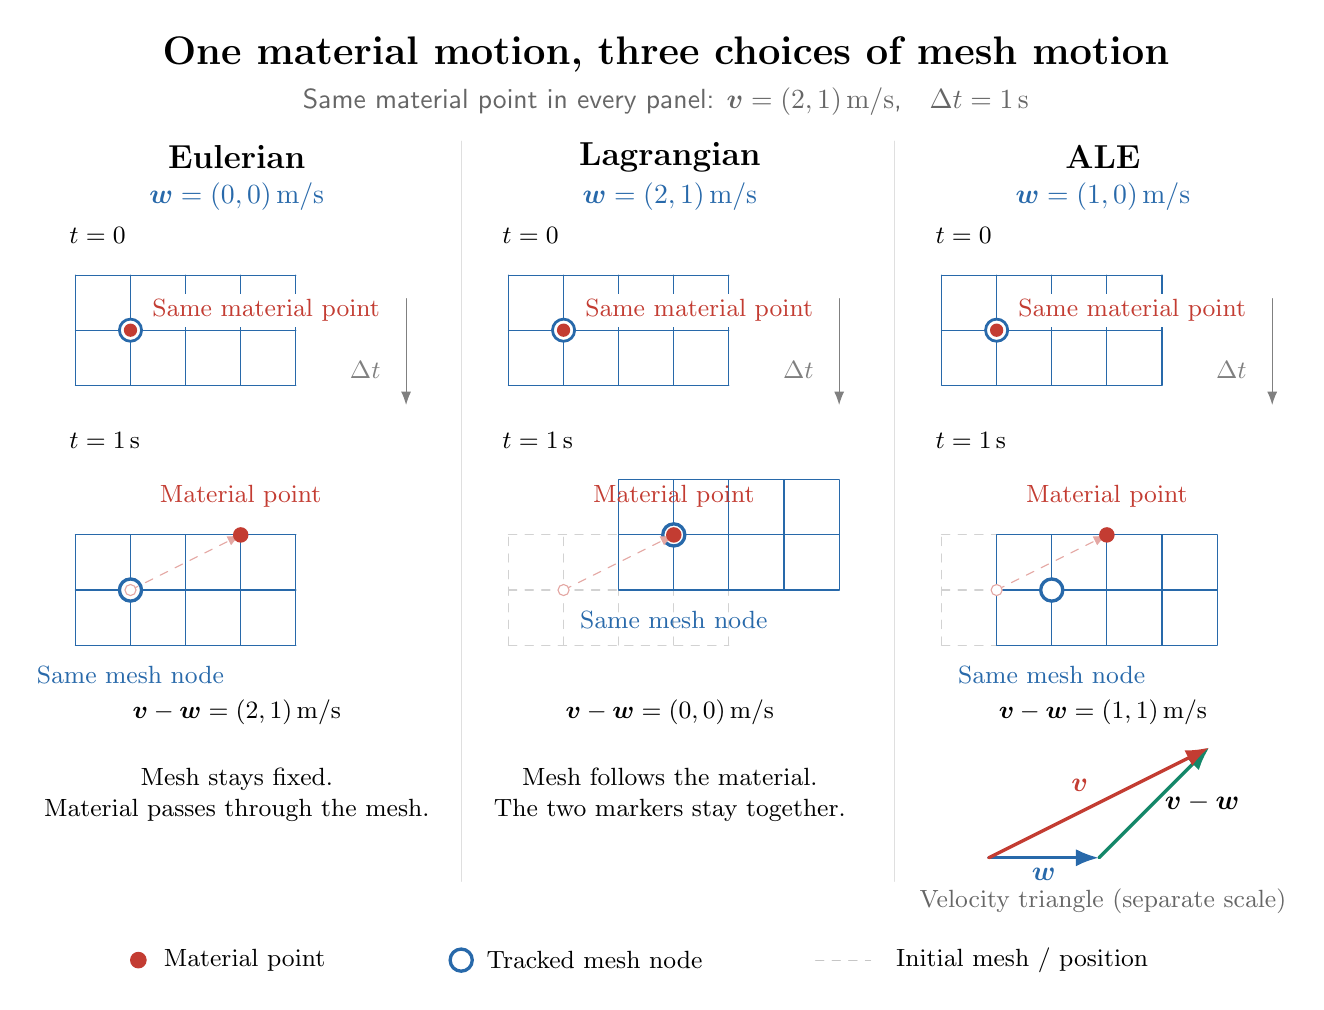
\begin{tikzpicture}[>=Latex,font=\sffamily,line cap=round]
\node[font=\Large\bfseries] at (7.7,8) {One material motion, three choices of mesh motion};
\node[text=gray!80!black] at (7.7,7.4) {Same material point in every panel: $\boldsymbol v=(2,1)\,\mathrm{m/s}$,\quad $\Delta t=1\,\mathrm s$};
% One metre is represented by 0.7 cm in every spatial diagram.
\foreach \offset/\title/\sx/\sy/\w/\rel in {
0/Eulerian/0/0/{(0,0)}/{(2,1)},
5.5/Lagrangian/1.4/0.7/{(2,1)}/{(0,0)},
11/ALE/0.7/0/{(1,0)}/{(1,1)}}{
\begin{scope}[shift={(\offset,0)}]
\node[font=\large\bfseries] at (2.25,6.7) {\title};
\node[mesh] at (2.25,6.2) {$\boldsymbol w=\w\,\mathrm{m/s}$};
\node[anchor=west,font=\small\bfseries] at (0,5.7) {$t=0$};
\begin{scope}[shift={(.2,3.8)}]\draw[mesh,step=.7,thin] (0,0) grid (2.8,1.4);\end{scope}
% Highlight a specific mesh node, initially coincident with the material point.
\draw[mesh,fill=white,line width=1pt] (.9,4.5) circle (4pt);
\fill[particle] (.9,4.5) circle (2.4pt);
\node[particle,anchor=west,font=\small,fill=white,inner sep=2pt] at (1.1,4.75) {Same material point};
\draw[->,gray] (4.4,4.9)--(4.4,3.55);
\node[anchor=east,font=\small,text=gray] at (4.2,4) {$\Delta t$};
\node[anchor=west,font=\small\bfseries] at (0,3.1) {$t=1\,\mathrm s$};
% Old mesh is retained as a light reference; current mesh is solid blue.
\begin{scope}[shift={(.2,.5)}]\draw[gray!35,dashed,step=.7,thin] (0,0) grid (2.8,1.4);\end{scope}
\begin{scope}[shift={(\sx,\sy)}]
\begin{scope}[shift={(.2,.5)}]\draw[mesh,step=.7,thin] (0,0) grid (2.8,1.4);\end{scope}
\draw[mesh,fill=white,line width=1.2pt] (.9,1.2) circle (4pt);
\end{scope}
\draw[particle!45,dashed,->] (.9,1.2)--(2.3,1.9);
\draw[particle!45,fill=white] (.9,1.2) circle (2pt);
\fill[particle] (2.3,1.9) circle (2.8pt);
\node[particle,anchor=south,font=\small] at (2.3,2.12) {Material point};
\node[mesh,anchor=north,font=\small] at (.9+\sx,.5+\sy-.14) {Same mesh node};
\node[font=\small] at (2.25,-.35) {$\boldsymbol v-\boldsymbol w=\rel\,\mathrm{m/s}$};
\end{scope}}
\draw[gray!25] (5.1,-2.5)--(5.1,6.9);
\draw[gray!25] (10.6,-2.5)--(10.6,6.9);
\node[align=center,font=\small] at (2.25,-1.4) {Mesh stays fixed.\\Material passes through the mesh.};
\node[align=center,font=\small] at (7.75,-1.4) {Mesh follows the material.\\The two markers stay together.};
% Velocity triangle, detached from the spatial diagrams above.
\begin{scope}[shift={(11.8,-2.2)}]
\draw[mesh,->,very thick] (0,0)--(1.4,0) node[midway,below] {$\boldsymbol w$};
\draw[draw=relative,->,very thick] (1.4,0)--(2.8,1.4) node[midway,right] {$\boldsymbol v-\boldsymbol w$};
\draw[particle,->,very thick] (0,0)--(2.8,1.4) node[midway,above left] {$\boldsymbol v$};
\end{scope}
\node[font=\small,text=gray!80!black] at (13.25,-2.75) {Velocity triangle (separate scale)};
\draw[particle,fill=particle] (1,-3.5) circle (2.8pt);
\node[anchor=west,font=\small] at (1.2,-3.5) {Material point};
\draw[mesh,fill=white,line width=1.2pt] (5.1,-3.5) circle (4pt);
\node[anchor=west,font=\small] at (5.3,-3.5) {Tracked mesh node};
\draw[gray!45,dashed] (9.6,-3.5)--(10.3,-3.5);
\node[anchor=west,font=\small] at (10.5,-3.5) {Initial mesh / position};
\end{tikzpicture}
\end{document}
